\section{$\mu$P4C Compiler}
\label{section-mp4c-compiler}


\subsection{Parser Block Transformation}
\label{subsection:parser-block-transformation}
P4 parser blocks describe parse graphs as state machines.
Real target devices contain programmable parser module that can be programmed using parse graphs.
From the design of programmable parser~\cite{6665172}, we make following observations.
Programmable parsers are implemented using buffer, state machine logic, Ternary Content-Addressable Memories (TCAM) and Action RAM. 
TCAM matches values of current state, fields or variables to identify next state. 
Based on match, headers are copied from bit stream and current state is modified.
Programmable parsers essentially perform repeated match and action.
Also, we note that network packets are of finite length, hence they can be parsed in a finite number of ways.
Successful parsing of a packet is essentially finding a match for a finite number of bytes from finite set of values.
However, we need to extract all the bytes that might be required to perform match-actions from packets' bit streams.


We compute number of bytes required to extract in section~\ref{subsubsection:computing-size-of-byte-array}, followed by an approach to convert parser without loops and variable length headers, called \textit{simple parsers}, into a series of match-action tables.
Next, we explain loops unrolling and variable length headers removal techniques transforming every parser into a simple parser.
Finally, we discuss an optimization to reduce number of MATs to one.


\subsubsection{Computing Size of Byte Array}
\label{subsubsection:computing-size-of-byte-array}
% Every \emph{extract} method call statement in parser states advances bit index by number of bits equal to the size of the header type of the instance passed as the argument.
We perform symbolic execution of parser, control and deparser blocks to determine size of byte array buffer by evaluating call statements of \emph{extract} and \emph{emit} methods of core library externs \emph{packet\_in} and \emph{packet\_out}, respectively.
The symbolic execution also tracks validity of header instances by evaluating \emph{setValid} and \emph{setInvalid} method calls of P4 header types.
Symbolic execution of a parser block enumerates every possible path from the start to the accept state in the parse graph and computes total number of bytes extracted on every path.
We define length $l_{p}(x)$ of a path $x$ from the start to the accept state in the parse graph of program $p$'s parser as total number of bytes extracted.
And, the input buffer size for program $p$'s parser as $\mathcal{I}(p) = \max_{x}\left\{l_{p}(x)\right\}$. 


Programs may increase or decrease size of packets, therefore, considering only parser buffer size is not enough.
We perform symbolic execution of control and deparser blocks to determine maximum increase and decrease in packet size by the program.
We evaluate header instances' setValid and setInvalid method call statements on every path of the control flow graph.
We define worst case scenarios to estimate increase and decrese of size of packets on the same control path.
To estimate maximum decrement, we consider that a packet contains all the header instances that are set to valid or invalid on a control path.
Similarly for maximum increment, we consider that a packet does not contain any header instance that is set to valid or invalid on a control path. 
We denote increase and decrease in packet size on a path $x$ of control block of program $p$ using $i_{p}(x)$ and $d_{p}(x)$.
We define them as sum of sizes of all the header instances set valid and invalid on the path, respectively.
Header instances not emitted in any paths of deparser block by extracted by a parser state decrease packets size. 
For every path $x$, $d_{p}(x)$ is increamented by the size of such header instances. 
We define maximum decrease and increase in packet size by program $p$ as $\delta(p)$ and $\Delta(p)$, as shown in (\ref{decrease}) and (\ref{increase}).


\begin{align}
\delta(p)\; =& \;  \max_{x} \left\{ d_{p}(x) \right\} \label{decrease} \\
\Delta(p) \; =& \; \max_{x} \left\{ i_{p}(x) \right\} \label{increase}
\end{align}

To process packets by a sequence of $N$ programs, we define extract length, $\mathcal{E}l_{S}$ and buffer length $\mathcal{B}l_{S}$, as shown in (\ref{extract-length-seq}) and (\ref{buffer-length-seq}).
$\mathcal{E}l_{S}$ denotes the maximum number of bytes that may be extracted as cumulative effect of deparsers and parsers of all the program in a sequence.
$\mathcal{B}l_{S}$ denotes the maximum number of bytes that may be emitted as cumulative effect of the deparsers of all the programs in a sequence.
Similarly, we define extract length, $\mathcal{E}l_{P}$ and buffer length $\mathcal{B}l_{P}$, as shown in (\ref{extract-length-par}) and (\ref{buffer-length-par}), to process packets by $N$ programs in parallel.
\begin{align}
\mathcal{E}l_{S} \; =& \; \max_{i} \left\{ \left( \sum_{j=0}^{j<i} \delta(j) \right)+ \mathcal{I}(i) \right\},&\;\;\;i  \in [0,N] \label{extract-length-seq} \\
\mathcal{B}l_{S} \; =& \; \left( \sum_{i=0}^{N} \Delta(i) \right)+ \mathcal{E}l_{S} & \label{buffer-length-seq} \\
\mathcal{E}l_{P} \; =& \; \max_{i} \left\{ \mathcal{I}(i) \right\},&\;\;\;i  \in [0,N] \label{extract-length-par} \\
\mathcal{B}l_{P} \; =& \; \max_{i} \left\{ \mathcal{I}(i) + \Delta(i) \right\},&\;\;\;i  \in [0,N]  \label{buffer-length-par}
\end{align}


\subsubsection{Simple Parser to MATs}
\label{subsubsection:simple-parser-to-mats}
% We create action stage using parserStatements and match stage using ~\texttt{transitionStatement}.
Every path enumerated by symbolic execution of a parser consists of evaluated instances of the parser states.
A parser state can be a part of multiple paths, thereby having multiple instances.
% Every evaluated instance of a state provides a set of extracted (valid) header instances and their start bit indices corresponding to the state and the path.
P4 parser states consist of ~\emph{parser-Statements}  and \emph{transition\-Statement}.
The select expression in transition statement could be a header field, metadata or local variable declared in the parser.
The value of select expression of a state may depend on its ancestors' parser statements. <<as shown in diagram>>
Therefore, we perform Forward Substitution on select expressions in evaluated instances of states
% (https://dl.acm.org/citation.cfm?id=7904)
on each path and eliminate such data dependency.

We synthesise local binary variables, called \emph{visit},  for each parser state to track the state transition of the parser's FSM.
For every evaluated instance of a parser state, we synthesise an action comprising its parser\-Statements and replace extract method call statements to assignment statements.
The assignment statements copies bytes from the buffer array to header instances' fields according to their sizes.
Next, we add pop method call with the header size as the argument to remove the header from the byte array.
We insert setValid method call statement for the extracted header instances.
We add an assignment statement to set visit variable associated with the parser state.

\begin{figure*}[!h]
    \begin{subfigure}[b]{0.3\linewidth}
        \centering
        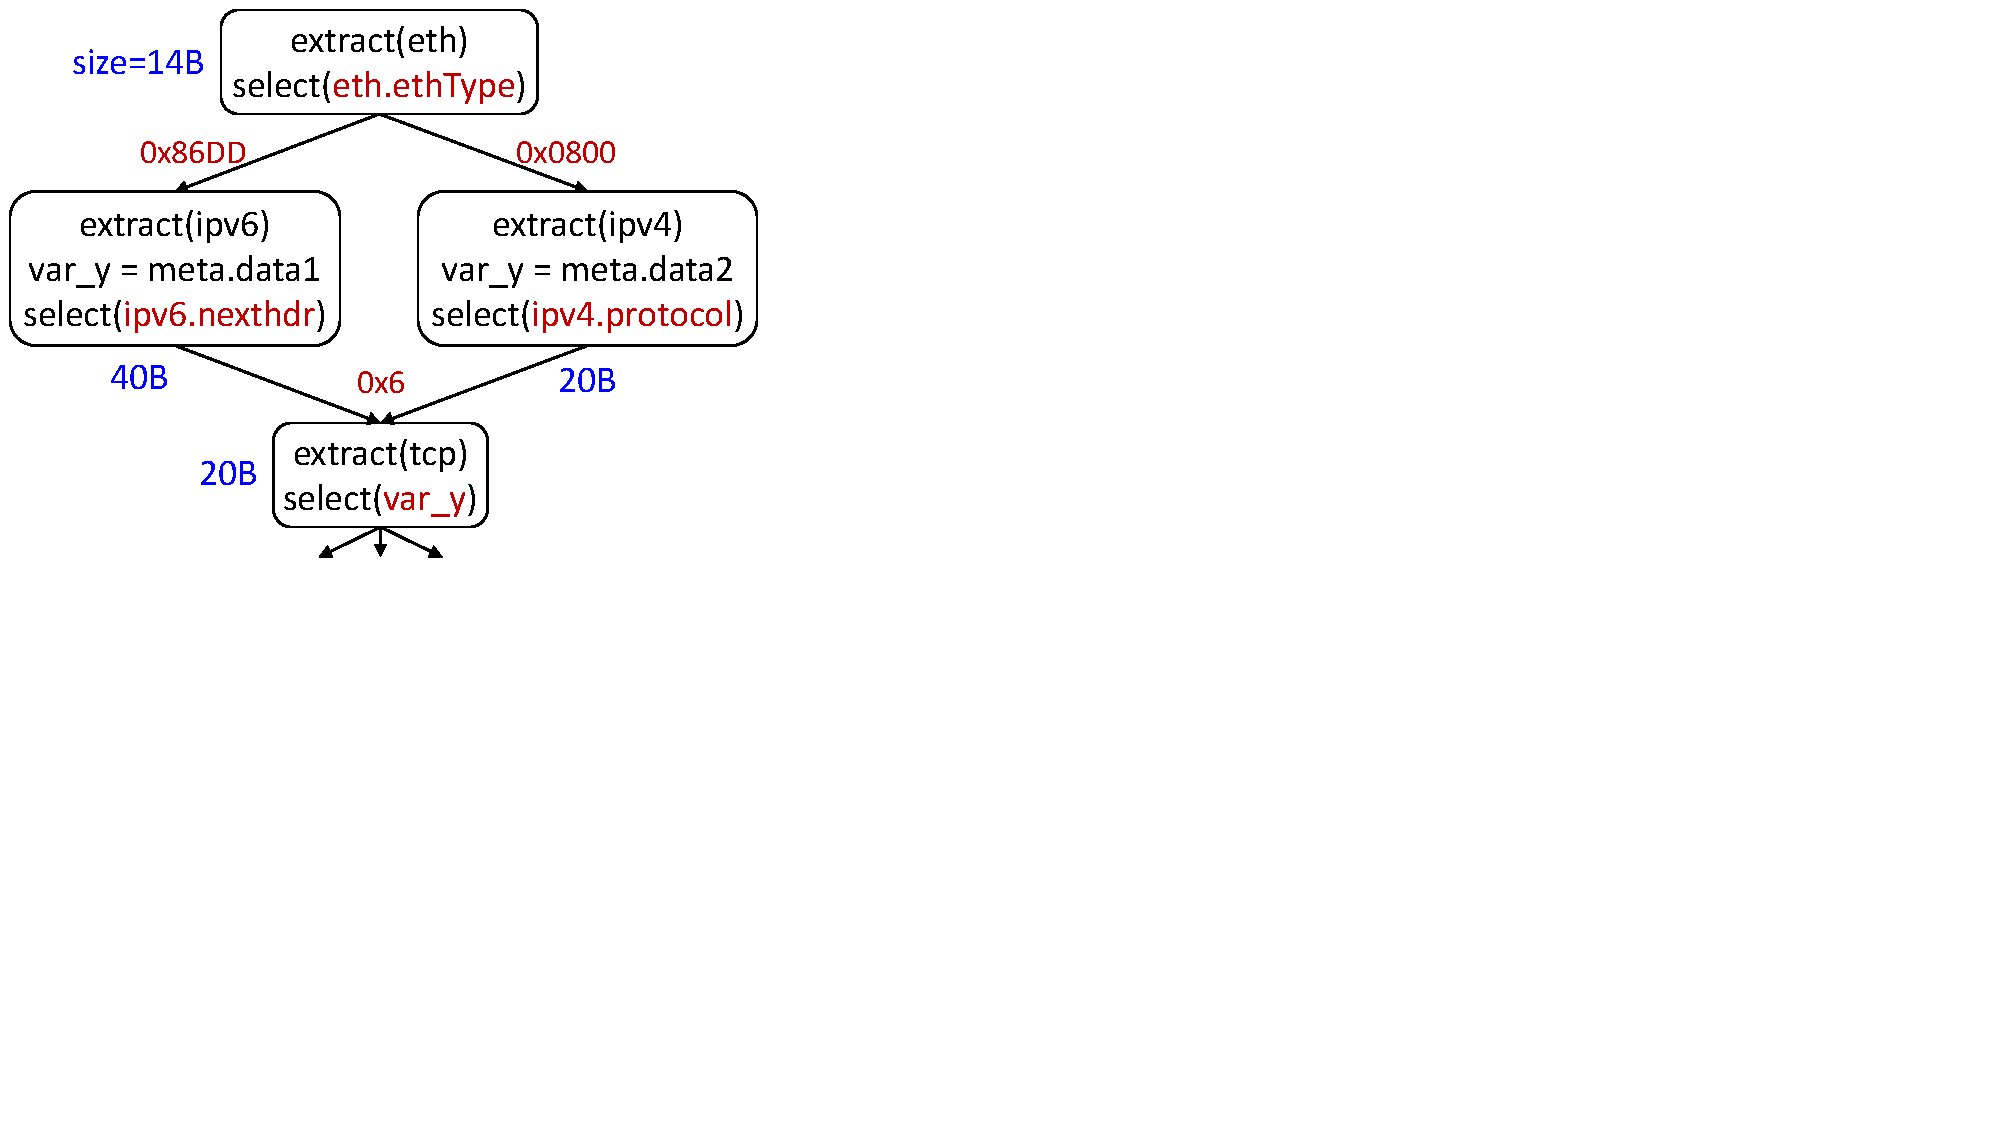
\includegraphics[trim=4 270 596 0, clip,scale=0.4]{parser-transformation-example}
        \caption{An example P4 Parser}
        \label{subfig:parser}
    \end{subfigure}
    \begin{subfigure}[b]{0.3\linewidth}
        \centering
        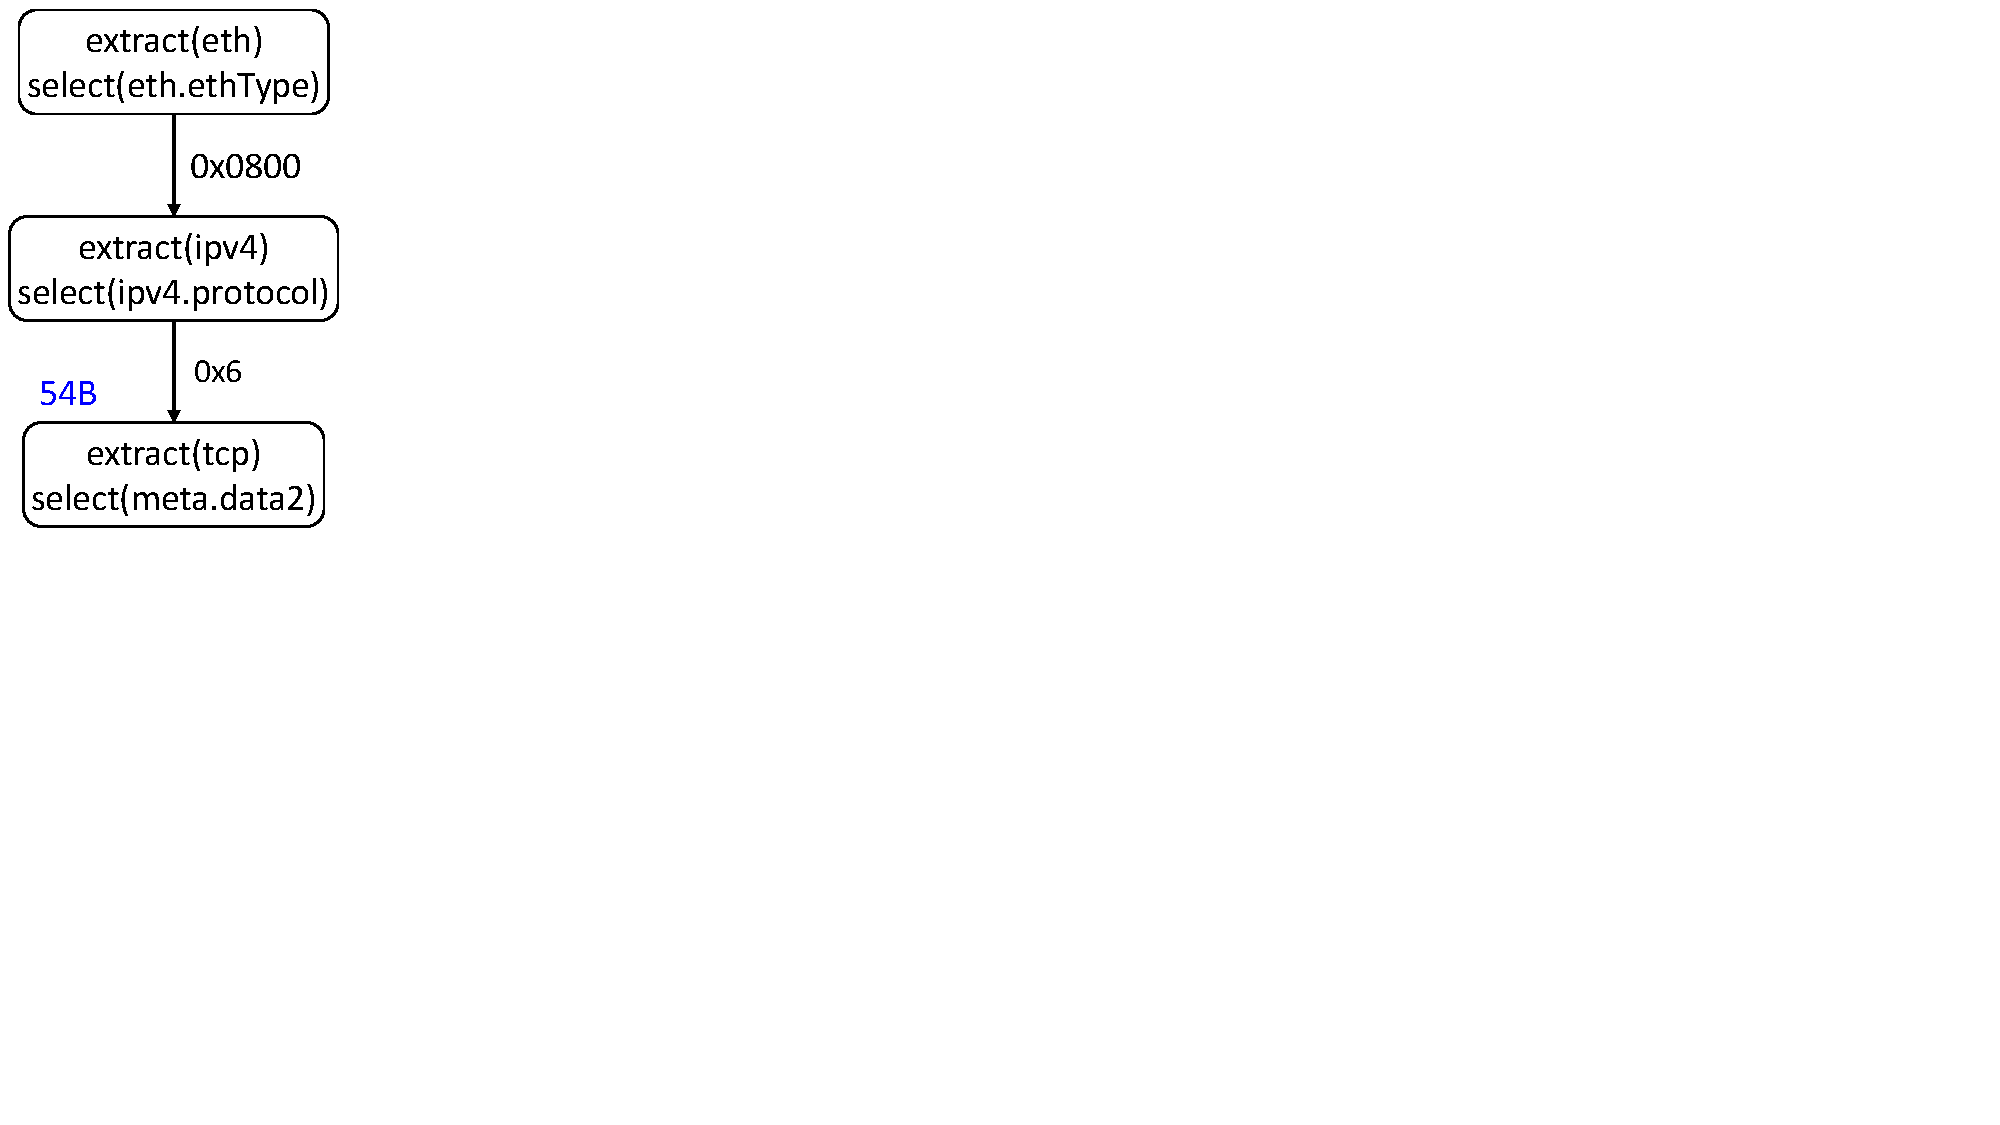
\includegraphics[trim=4 285 796 0, clip,scale=0.4]{parser-example-se-1}
        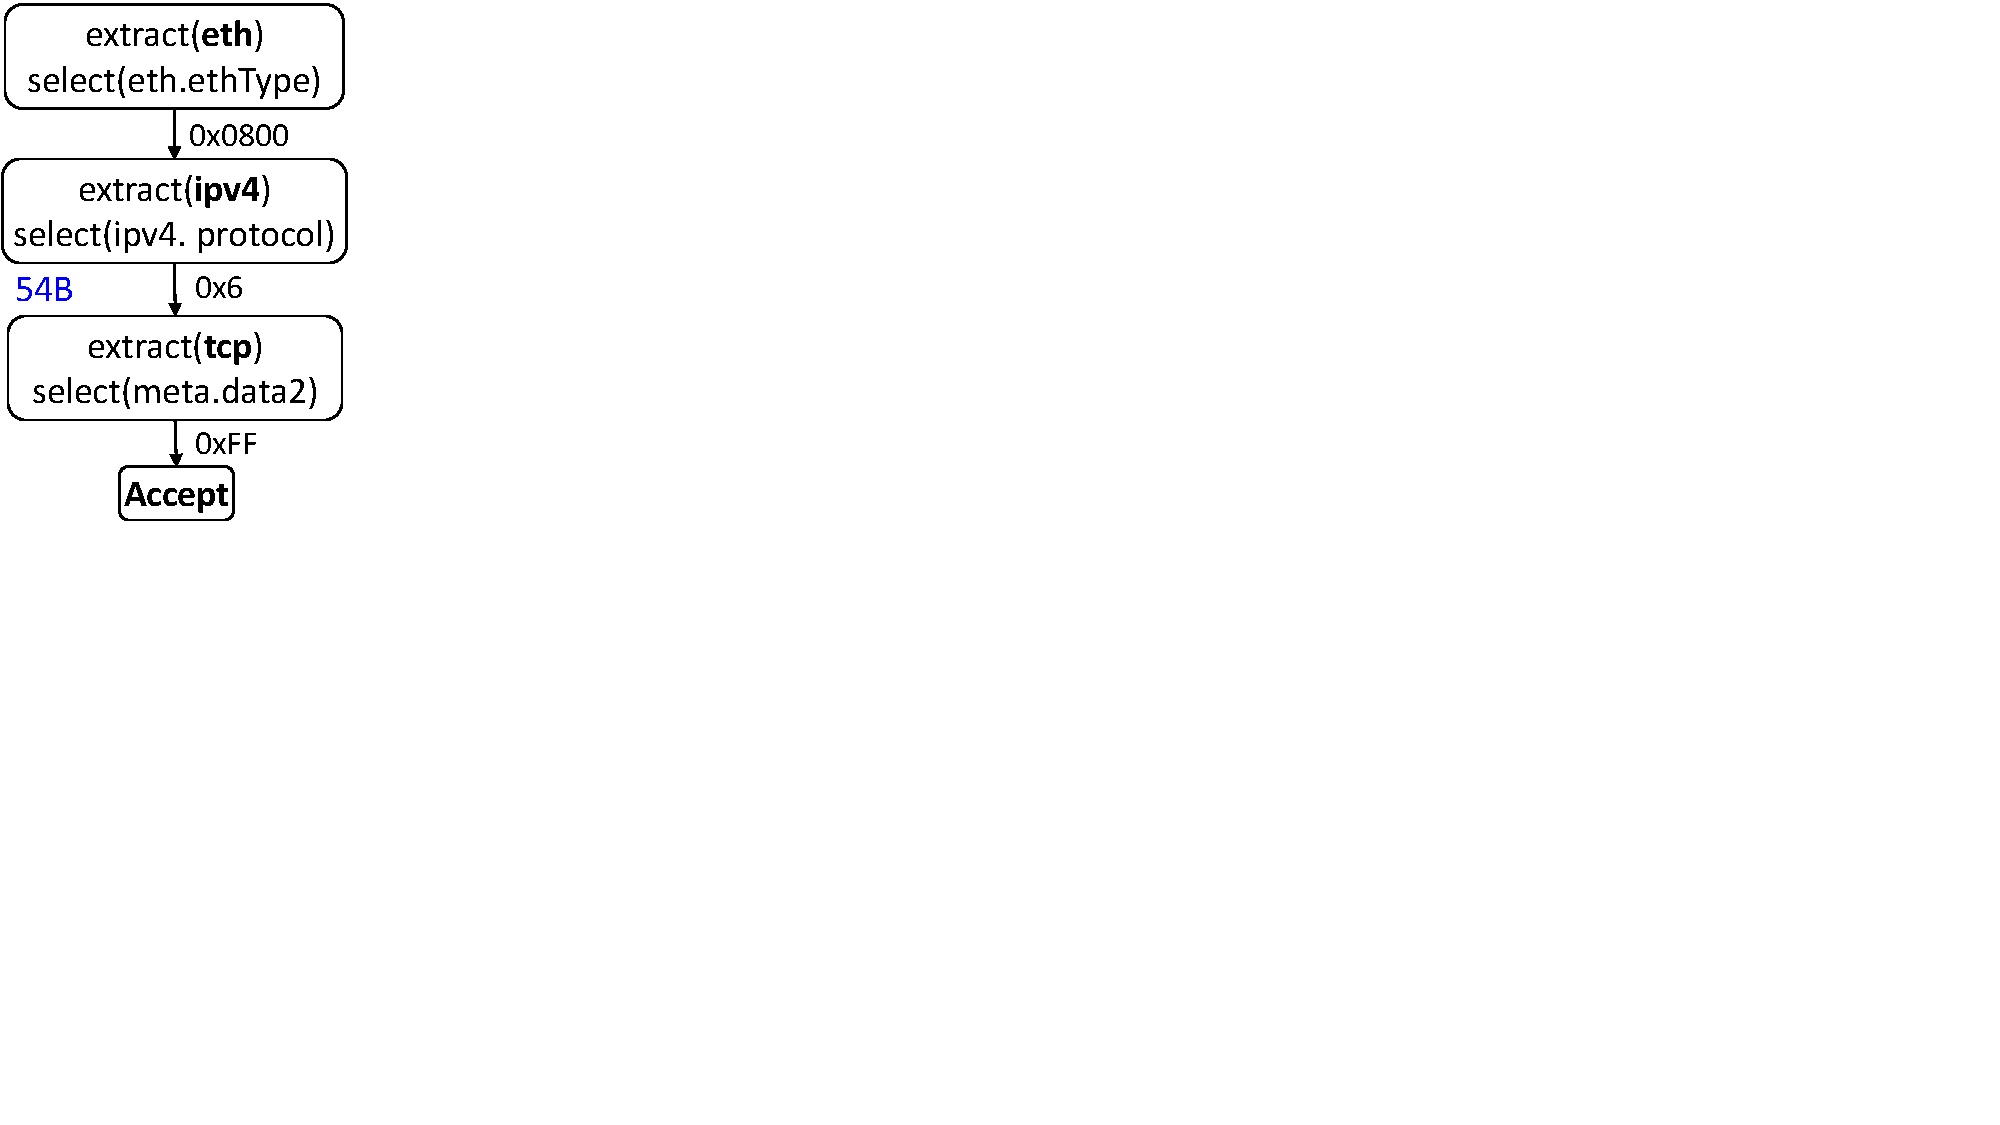
\includegraphics[trim=4 285 796 0, clip,scale=0.4]{parser-example-se-2}
        \caption{Parser Symbolic Execution}
        \label{subfig:parser-symbolic-execution}
    \end{subfigure}
    \begin{subfigure}[b]{.4\linewidth}
\begin{lstlisting}[frame=none]
control Pipe(inout hdr_t hdrs, out bit<16> nexthop_id, inout sm_t sm) {
  action process(bit<16> nh) {
    hdrs.ipv4.ttl = hdrs.ipv4 - 1;
    nexthop_id = nh;// setting out param
  }
  table ipv4_lpm_tbl {
    key = { hdrs.ipv4.dstAddr : lpm } 
    actions = { process; }
  }
  apply { ipv4_lpm_tbl.apply(); }
}
\end{lstlisting}
\caption{Match-Action Control Block}
\label{subfig:parser-symbolic-execution}
\end{subfigure}
\caption{Parser to Control Block Transformation}
\label{fig:parser-to-control-block-transformation}
\end{figure*}

For every parser state, we create a match key comprising key-fields from sets of keys. 
$(1)$ $visit$ variable assocociated with the set of all its ancestors and the state itself and
$(2)$ union of select expression of all of its evaluated instances.
In most cases, the union of select expression would have a single key-field, unless forward substitution has produced different expressions in the state's evaluated instances.

The \emph{start} being a special state has only one evaluated instance.
We create an action, called \emph{start\_action}, from the only instance of the start state.
Next, we visit parser states in topological order. 
We create match key for the current parser state as described above.
The match-key entries are created using keysetExpression and all possible paths represented to the state encoded using visit bit vector.
For each match key entry, we use appropriate action synthesised by next state's evaluated instance.

The apply body of the control block consists of an action call invalidating all the header instances, followed by the start\_action call and apply calls to the MATs created for parser states in topological order.



\subsubsection{Variable Length Headers and Loops Elimination}
\label{variable-length-headers-loops-and-elimination}
The two-argument extract method is replaced with a synthesised sub-parser with three arguments.
First to arguments are the same as two-argument extract method and the third arguments is maximum size of variable field.
The start state of the sub-parser contains a transition\-Statement with a select\-Expression.
The sub-parser contains a state for each possible value of variable field size that extracts constant number of bits using single argument extract method and transits to accept state.
The select\-Expression of the start state uses the variable field size parameter(the second parameter) to match on and transit to the corresponding next state.




\subsection{Deparser Block Transformation}
\label{subsection:deparser-block-transformation}
Recall that deparser blocks are specialized control blocks having packet\_out extern as one of the arguments.
The extern's emit method inserts bits on packets' bit-stream, if the header instance provided in the argument is valid, else no operation is performed.
We precisely perform the same operation on byte array buffer, but first we create a match-action table to push fixed number of bytes on the byte array buffer.
Recall that the program's parser transformation pops the total number of extracted bytes from the array buffer.
If the program's parser extracts less than $\mathcal{E}l$ for a particular packet, there are valid data on byte array.

The key of the table are created using valid bit of each header instance.
The table contains entries enumerating all possible combination of validity of the headers and action corresponding to each match key value to push the number of bytes equals to sum of lengths of all valid headers.


The deparser block may contain P4 language constructs like \emph{if-else} and \emph{switch} statements in addition of emit method call statements.
Therefore, deparser block may have multiple execution paths emitting the same header instances. 
We derive a directed-acyclic-graph, called \emph{emit graph}, with each node representing a emit call from the control flow graph of the deparser control block.
We synthesise a match-action table for every emit method call in deparser blocks.
Similar to one bit $visit$ variable for parser states, we create one bit variable, \emph{emit}, for each node in the emit graph.
The match key for the match-action table for an emit node comprises valid bit of the header instances passed as argument to its ancestors.
In addition, the match key includes $emit$ variables associated with the ancestors.
The idea behind introducing $emit$ variable is to record execution of previous emit calls in the control path and copy header instance  of emit call at appropriate location in the byte array buffer.



\subsection{(De)parser Control Block Optimization}
The transformation of parser and deparser blocks into match-action control blocks induces huge cost in terms of number of binary variables in data plane and multiple match-action tables.
Also, number of entries in the tables are of exponential order of binary variable fields in the tables.
In this section, we describe optimization methods to reduce per state match-action tables in transformed parser blocks into a single match-action table and eliminate all the binary variables.
 
 


\subsection{Real-Target Specific Transformation}
The architectures or real target devices specify target-specific externs, pipeline model and constraints in programmable blocks in pipelines.



\subsubsection{Control Block Pipeline Split}


